\documentclass[pdflatex,sn-mathphys-num]{sn-jnl}% Math and Physical

\usepackage{hyperref} % For clickable links
\usepackage{graphicx}%
\usepackage{multirow}%
\usepackage{amsmath,amssymb,amsfonts}%
\usepackage{amsthm}%
\usepackage{mathrsfs}%

\usepackage{xcolor}%
\usepackage{textcomp}%
\usepackage{manyfoot}%
\usepackage{booktabs}%
\usepackage{algorithm}%
\usepackage{algorithmicx}%
\usepackage{algpseudocode}%
\usepackage{listings}%
\usepackage{float}

\raggedbottom
%%\unnumbered% uncomment this for unnumbered level heads


\begin{document}

\author*[1]{\fnm{Telmo} \sur{Miguel-Medina}}\email{tmiguel@ubu.es}

\affil[1]{\orgdiv{Electromechanical Engineering Department}, \orgname{University of Burgos}, \city{Burgos}, \country{Spain}}

\title[From Code Repository to Research Infrastructure]{From Code Repository to Research Infrastructure: Evaluating GitHub for Managing the Scientific Research Lifecycle}

\abstract{
\textbf{Aims:} Research artifacts are usually managed across disconnected tools, with weak traceability of the process that produced the outputs. We ask to what extent GitHub's native functionalities can serve as an integrated infrastructure for managing the scientific research process across the lifecycle.

\textbf{Methods:} A hybrid design: a bibliometric analysis of a 5{,}139-work OpenAlex and arXiv corpus (2008--2025) mapped onto lifecycle stages; a structured review of 67 studies yielding fifteen research management requirements; a reproducible four-level assessment of GitHub's 68 native capabilities against them; a reference architecture and reusable template synthesised from the mapping; and a self-referential implementation, evaluated on six dimensions and re-instantiated on a second, unrelated project.

\textbf{Results:} The literature is output-biased --- data management and analysis dominate (50.8\% and 41.9\% of the corpus) against 3.7\% for idea and question formulation. GitHub supports 13 of 15 requirements at partial or better and 7 directly (mean 2.43 of 3 for the fourteen core requirements), none unsupported, but support is direct where research resembles software engineering and only partial or limited for the research-specific traceability of questions, decisions and provenance --- the requirements the literature also under-serves (1.67 versus 2.50). Five requirements need external infrastructure. A 15-component architecture with four mandatory conventions and a 33-file template operationalise what is covered; in the self-referential implementation 13 of 15 components were exercised and the six-dimension score reached 1.86 of 2 (usability lowest at 1.50), and a retrospective instantiation on an unrelated clinical-machine-learning project reproduced the profile.

\textbf{Conclusion:} GitHub can serve as an integrated coordination and traceability \emph{layer} for a substantial part of the research lifecycle --- strong from execution to output, weak upstream, and dependent on complementary infrastructure for preservation and large data. It maps the research-process-management gap rather than closing it.

\keywords{research infrastructure, research process management, GitHub, research lifecycle, reproducibility, open science}
}

\maketitle


\section{Introduction}\label{sec:intro}

\subsection{Complexity and artifact proliferation in modern research}\label{sec:complexity}

A contemporary research project is a chain of interdependent objects: a research question, a protocol, a literature corpus, data, analysis code, a computational environment, intermediate results, figures, tables, a manuscript, a publication, released software and supplementary material. These objects evolve continuously and are produced by distributed, often multidisciplinary teams. Computational and data-intensive research has amplified both the number of artifacts and the need to keep them consistent with one another \citep{liew2016,liu2015,mattoso2015}.

\subsection{Fragmentation of research-process management}\label{sec:fragmentation}

In common practice these artifacts and the activities that generate them are spread across disconnected systems: email, cloud storage, local folders, spreadsheets, reference managers, statistical software, code repositories, task managers and manuscript editors. Each tool serves its local function, but the coordination layer between them is largely absent. Reviews of research data management, scholarly infrastructure and post-award reporting repeatedly associate this fragmentation with weak decision traceability, incomplete process documentation, inconsistent versioning, limited provenance and low project visibility \citep{perrier2017,donner2022,crane2023,tutko2022}.

\subsection{Managing the process, not only archiving the outputs}\label{sec:process}

Two decades of work on scientific workflow systems, provenance, research data management, virtual research environments and open-science platforms have produced mature evidence on \emph{output} stewardship --- repositories, persistent identifiers, curation, dissemination \citep{davidson2008,perez2018,ho2025,kirkham2020,mayernik2017}. The management of the research \emph{process} that produces those outputs --- planning, question formulation, decision tracking, cross-stage coordination --- has received comparatively little systematic, quantitative attention \citep{cox2018,holler2022,devkota2026}.

\subsection{Prior reviews, by strand}\label{sec:related}

The evidence base is a set of partially connected review literatures. \emph{Scientific workflow systems} are the most surveyed: recurring reviews catalogue execution engines, scheduling and data-intensive orchestration \citep{liew2016,liu2015,mattoso2015}, but they take the research question, the analysis plan and the decisions behind a pipeline as given and start at the executable graph. \emph{Provenance} research extends this with models for capturing and querying the lineage of workflow runs \citep{davidson2008,oliveira2018,perez2018}; systematic reviews of provenance systems repeatedly note that coverage stops at data and computation and rarely reaches the upstream intellectual choices. \emph{Research data management} reviews document institutional services, roles and lifecycle models for curating and sharing data \citep{perrier2017,donner2022,cox2018,ho2025}, again concentrating on data as an output rather than on the process that generates it. \emph{Research information systems} and knowledge-graph reviews describe institutional infrastructures for recording researchers, projects and outputs for reporting and evaluation \citep{mayernik2017,haris2026}, at an administrative rather than a project-working granularity. \emph{Open-science} syntheses map practices and incentives for transparency, preprints and reproducible reporting \citep{klebel2025,kirkham2020}. Finally, a \emph{version-control-in-research} strand --- mostly guidance and case reports rather than reviews --- argues that Git and GitHub can carry collaborative, reproducible research \citep{sandve2013,blischak2016,wilson2017,braga2023}. This study cuts across these strands: it treats the research \emph{process} as the object of management and asks how far one widely available platform can serve the requirements they each touch but none addresses as a whole.

\subsection{Code-hosting platforms beyond software}\label{sec:github}

GitHub already provides primitives for coordination, versioning, issue tracking, structured discussion, review and automation. Guidance and case studies describe its use for versioned, collaborative and reproducible research in computational biology \citep{sandve2013,blischak2016,perezriverol2016}, ecology and evolution \citep{braga2023}, laboratory research \citep{chen2025}, and for developing community data standards \citep{crystalornelas2021}; its footprint in the scholarly record is itself growing and measurable \citep{escamilla2022}. Yet this evidence is case-based, and studies that mine GitHub as research data caution that its use is heterogeneous and often shallow \citep{kalliamvakou2016,trisovic2022}. Whether GitHub's primitives can be organised into an infrastructure for managing the research process, and which lifecycle stages such an infrastructure can actually cover, has not been established on an evidentiary basis.

\subsection{Aim and research questions}\label{sec:rqs}

The aim of this study is to characterise the literature on digital infrastructure for research-process management, derive a lifecycle-structured set of research management requirements, determine quantitatively how far GitHub's native functionalities cover them, consolidate the covered functionalities into a reusable reference architecture and template, and probe feasibility through a self-referential implementation. The study does not claim that GitHub replaces specialised research infrastructure.

\begin{description}
  \item[RQ1] How has the literature on digital infrastructure for managing the research process evolved in volume, disciplines, venues and thematic structure, and which lifecycle stages are under-represented?
  \item[RQ2] What research project management requirements across the research lifecycle can be derived from this literature?
  \item[RQ3] To what extent, with what support level and limitations, do GitHub's native functionalities cover these requirements, and how is coverage distributed across lifecycle stages?
  \item[RQ4] How can the covered functionalities be organised into a coherent reusable reference architecture and project template?
  \item[RQ5] What does a self-referential implementation, together with the reusable template, reveal about feasibility, traceability gains and limitations relative to a fragmented workflow?
\end{description}


\section{Materials and Methods}\label{sec:methods}

\subsection{Overall design}\label{sec:design}

The study is a multi-method evidence synthesis with three coupled components: a bibliometric analysis of the field (RQ1); a structured requirement extraction and a reproducible requirement--functionality coverage analysis (RQ2, RQ3); and a design synthesis with a single self-referential feasibility test (RQ4, RQ5). All datasets, coding sheets, mapping tables and analysis scripts are openly available (Section~\ref{sec:data-availability}); every table and figure in this paper is regenerated by a versioned script from those inputs.

\subsection{Bibliometric corpus and analysis (RQ1)}\label{sec:m-biblio}

The primary corpus was built from OpenAlex, which indexes journal articles, conference papers and preprints with abstracts, concepts and citations and is fully reproducible from a published query. Fifteen \texttt{title\_and\_abstract} queries were run, grouped in four strands: core process management (\emph{``research project management''}, \emph{``research workflow''}, \emph{``research lifecycle''}, \emph{``scientific workflow''} and near-variants), data management and open science (\emph{``research data management''}, \emph{``open science''}, \emph{``reproducible research''}), version control in research (\emph{github}, \emph{``version control''} + \emph{research}), and research environments (\emph{``virtual research environment''}, \emph{``science gateway''}, \emph{``research information system''}). All were filtered to \texttt{2008--2025} and to document types article, review and proceedings-article, returning 6{,}512 hits and 5{,}936 unique works. Five narrower abstract- and title-scoped arXiv queries (\emph{``version control''}, \emph{github} within \texttt{cs.DL/SE/CY/DC}, \emph{``scientific workflow''}, \emph{``research software''}, \emph{``reproducible research''}) added 462 preprints, for 6{,}398 input records. De-duplication removed 1{,}167 data- and software-repository deposits (Zenodo, Figshare and similar, by an explicit source list), 29 duplicate DOIs, 9 duplicate title--year pairs and 31 no-DOI rows matching a DOI row on title and year, yielding a corpus of \textbf{5{,}139 works} (OpenAlex 4{,}689, arXiv 426, both 24).

As an independent coverage check, the same four query strands were run in Scopus (\texttt{TITLE-ABS-KEY}, document types article/review/conference paper) and Web of Science (\texttt{TS=} Topic), returning 18{,}250 raw and 13{,}586 de-duplicated in-window records. These share \textbf{22\% of their DOIs} with the OpenAlex/arXiv corpus; inspection of the non-overlapping set shows it is dominated by recent bioinformatics and computer-science tool papers that cite a GitHub repository and mention ``workflow'' or ``reproducibility'' in passing --- the low-precision tail a title- and abstract-anchored search deliberately excludes --- rather than missed core literature on research-process infrastructure. A heuristic precision estimate for the broadest OpenAlex queries was $\approx 0.94$. OpenAlex plus arXiv was therefore retained as the primary corpus for openness and full query reproducibility; the raw Scopus and Web of Science exports are archived with the dataset record.

Analysis covered annual production, source and disciplinary profile, country distribution, and a keyword co-occurrence map. Corpus concepts and abstracts were then matched against an eleven-item lexicon of research-lifecycle stages (idea, question, planning, literature, methods, data, analysis, results, dissemination, outputs, governance) to produce a stage-hit profile. Because indexing of 2025 was incomplete at retrieval, growth statements use a 2008--2024 series.

\subsection{Structured review and requirement extraction (RQ2)}\label{sec:m-review}

The requirement extraction rests on a structured evidence base of \textbf{52 review, survey and synthesis papers} identified through a deep-search synthesis prioritising secondary literature, complemented by \textbf{15 purposively selected primary studies} of Git and GitHub use in research (case reports and mining studies spanning computational biology, ecology, geography and software-repository research). From this base, each documented literature challenge was traced to a management need and then to a derived requirement following the chain \emph{finding $\rightarrow$ problem $\rightarrow$ need $\rightarrow$ requirement $\rightarrow$ category}, with the supporting studies recorded per row. Seventeen requirement rows were extracted and consolidated, by thematic grouping and reconciliation with a provisional domain list, into a framework of fifteen requirements (RM1--RM15), each with a definition, expected capabilities, lifecycle stages, evidence, a category, a relative importance and its interdependencies with the others. Requirements rated of high importance but weak in literature attention were flagged as \emph{differentiators}. Extraction was performed by a single coder. To probe coding stability, all coded decisions in the study --- the seventeen requirement-row assignments, the fifteen support levels of Section~\ref{sec:m-catalogue} and the twenty-one evaluation sub-scores of Section~\ref{sec:m-eval} --- were subsequently re-coded independently from the same source material and rubric; exact agreement was 96\% (Cohen's $\kappa$ 0.83--1.00 by unit), and the two adjacent-category disagreements leave every figure reported here unchanged. The absence of a second \emph{human} coder remains a limitation (Section~\ref{sec:limitations}).

\subsection{GitHub capability catalogue and mapping rubric (RQ3)}\label{sec:m-catalogue}

GitHub's \emph{native} functionality was catalogued as \textbf{68 capabilities in twelve feature groups} (repositories and Git, Markdown and documentation, Issues, Projects, Milestones, Labels, Discussions, Branches, Pull Requests, Actions, Releases and tags, and access/identity). Marketplace and third-party applications were excluded; the one retained non-native item is the GitHub--Zenodo release webhook, the de facto standard bridge for persistent identification. Each capability records its function, research use, the durable record it leaves, its plan availability (verified against GitHub documentation) and its limitations.

Each requirement RM1--RM15 was then assigned the best support level GitHub's native functionality can reach with a reasonable implementation pattern, using a four-level rubric: \emph{Direct} (3) --- a native feature meets the requirement; \emph{Partial} (2) --- met with an additional process or convention on native features; \emph{Limited} (1) --- marginal support only; \emph{Not supported} (0). Every assignment carries an evidence note, the primary capabilities, an implementation pattern, and any external-tool dependency. A stricter variant capping convention-heavy support at Limited was scored as a robustness check.

\subsection{Coverage indicators (RQ3)}\label{sec:m-coverage}

From the mapping we computed the support distribution, the mean support overall and by requirement category, the mean for the differentiators versus the rest, the count of requirements needing external tools, and a lifecycle-coverage profile (support weighted by each requirement's applicability to each stage). Because one requirement (governance and sustainability) is only partly in scope, the headline mean is reported for the fourteen core requirements as well as for all fifteen.

\subsection{Reference architecture and template (RQ4)}\label{sec:m-arch}

The Direct- and Partial-support capabilities were synthesised into a layered reference architecture of named components, each a single GitHub configuration serving a set of requirements, together with the conventions that make generic features research-usable, a lifecycle model and seven workflow definitions. The architecture was operationalised as a discipline-independent GitHub template repository, with a manifest mapping every file to the components and requirements it serves.

\subsection{Self-referential implementation and evaluation (RQ5)}\label{sec:m-eval}

Following a self-referential design, the framework was applied to the development of this study; the repository is the evidence. The documentation, decision-log and version-control components were exercised natively throughout Phases 1--11. The publication phase then enacted the parts a single-author sprint had left configured: the repository was made public, and the study's own outstanding work was reorganised into twelve GitHub Issues on the configured Project and taken through one full Issue $\rightarrow$ branch $\rightarrow$ pull request $\rightarrow$ merge $\rightarrow$ Release cycle, moving the coordination layer from configured to exercised once. Each of the fifteen architecture components was then classified by implementation status (native, partial or planned). The framework was evaluated on six dimensions --- requirement coverage, traceability, documentation, organization, transparency, usability --- with 21 sub-scores on a 0/1/2 scale, each tagged by basis as observed, retrospective, design-support or planned; after the publication phase, 20 of the 21 are observed. As external-validity evidence, the template was additionally instantiated retrospectively on a completed, published clinical-machine-learning project in a different discipline, mapping each of RM1--RM15 onto a template mechanism. A conventional fragmented workflow was contrasted with the framework across six traceability and visibility dimensions.


\section{Results}\label{sec:results}

\subsection{Bibliometric map of the field (RQ1)}\label{sec:r-biblio}

The literature is an assembly of partially connected strands --- scientific workflow systems, research data management, provenance, research information systems, open science and version control --- rather than one field. In the 5{,}139-work corpus, annual output rises nearly tenfold between 2008 and 2024. Publications concentrate in computer science, library and information science and the biomedical literature; the leading venues after removing repository deposits are the \emph{International Journal of Digital Curation}, \emph{Concurrency and Computation}, \emph{Future Generation Computer Systems}, \emph{F1000Research} and \emph{PLoS ONE}, and the leading countries are the United States, Germany, the United Kingdom, China and the Netherlands. The keyword co-occurrence map (Figure~\ref{fig:coword}) shows the corpus spanning computer science, data science, knowledge management and the social sciences, with workflow, provenance and research data management as recurring bridging terms.

The stage-hit profile is markedly uneven (Table~\ref{tab:lifecycle}). Data management and analysis dominate (50.8\% and 41.9\% of the corpus); dissemination and coordination follow (24.4\% and 21.1\%); and idea and question formulation are at the bottom (3.7\%), with provenance at 7.0\%. A stage-level reading rates seven of fifteen lifecycle stages as thinly covered: idea, question, planning, ethics review, post-publication traceability, cross-stage coordination and governance. The structured review of 52 secondary studies reproduces the same bias independently.

\begin{figure}[h]
\centering
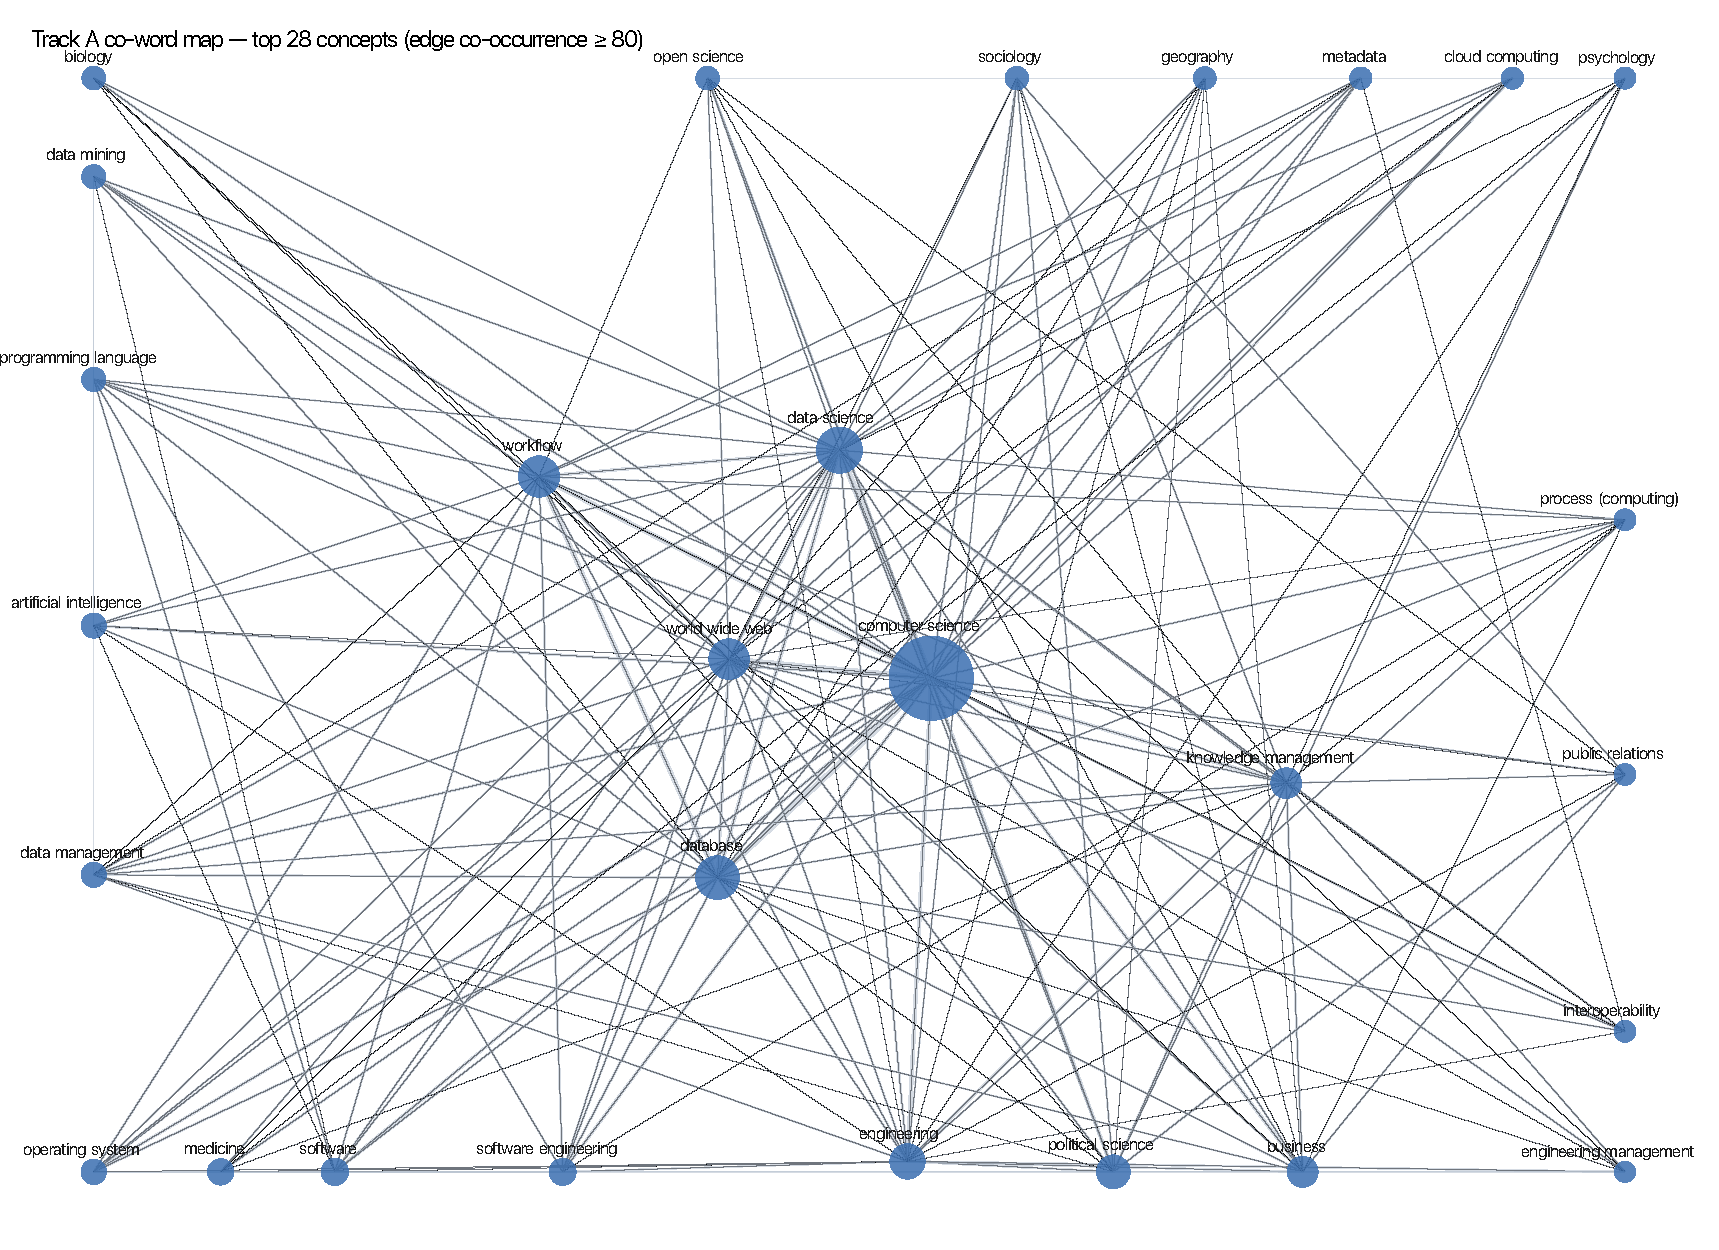
\includegraphics[width=\textwidth]{figures/coword_map.pdf}
\caption{Keyword co-occurrence map of the 5{,}139-work corpus (top concepts; edges are strong co-occurrences). The field spans computer science, data science, information management and the social sciences, bridged by workflow, provenance and research data management.}\label{fig:coword}
\end{figure}

\begin{table}[h]
\caption{Research-lifecycle stage coverage in the bibliometric corpus (RQ1). Share of the 5{,}139-work corpus whose concepts or abstract match the stage lexicon.}\label{tab:lifecycle}
\begin{tabular}{@{}lr@{\hskip 2em}lr@{}}
\toprule
Stage & \% of corpus & Stage & \% of corpus \\
\midrule
Data management        & 50.8 & Planning                 & 12.7 \\
Analysis / workflow     & 41.9 & Literature               & 10.0 \\
Dissemination           & 24.4 & Outputs / identification & 11.9 \\
Coordination            & 21.1 & Governance               & 10.9 \\
Methods / protocol      & 13.7 & Provenance               & 7.0  \\
                        &      & Idea / question          & \textbf{3.7} \\
\botrule
\end{tabular}
\end{table}

\subsection{Requirements and GitHub coverage (RQ2, RQ3)}\label{sec:r-coverage}

\paragraph{Requirements (RQ2).} Fifteen requirements were derived (Table~\ref{tab:requirements}), concentrated in traceability (four), documentation (three) and collaboration (two). Three requirements --- research planning (RM1), research-question management (RM2) and decision traceability (RM5) --- are of high importance yet weakly attended to in the literature; these differentiators define the gap the study targets. The requirements are interdependent: provenance (RM10) consumes RM2, RM4, RM5, RM8 and RM9, and transparency (RM11) is an emergent property of RM4, RM5, RM8 and RM10.

\paragraph{Coverage (RQ3).} GitHub supports \textbf{13 of 15 requirements at Partial or better and 7 at Direct}, with none unsupported. The mean support is \textbf{2.43 of 3} for the fourteen core requirements (2.33 for all fifteen). Support is Direct where research work resembles software engineering --- task management, review-based collaboration, communication, version control, documentation, transparency and automation, all with category means of 3.0 --- and Partial or Limited for research-specific traceability (RM2 Limited; RM5 and RM10 Partial), planning (RM1 Partial) and governance (RM15 Limited) (Table~\ref{tab:coverage}). The differentiator requirements have a mean support of \textbf{1.67 against 2.50} for the rest: the upstream gap seen bibliometrically in RQ1 reappears, independently, in GitHub's coverage.

Five requirements cannot be met by GitHub alone --- version control of large data (RM8), integration across heterogeneous tools (RM9), reproducibility (RM12), persistent identification and preservation (RM14) and governance (RM15) --- and require external infrastructure. The lifecycle-coverage profile is comparatively flat (weighted mean support 2.1--2.4 per stage) but lowest at idea (2.12) and question (2.25) and highest at literature, analysis and manuscript, echoing the RQ1 shape. Issues and the Git repository carry most of the framework; Projects, Actions, Discussions, Branches and Releases each contribute to only a few requirements. Under the stricter rubric the overall mean falls to 2.13, but the distribution (7 Direct, 3 Partial, 5 Limited, 0 unsupported) and the qualitative conclusion are unchanged.

\paragraph{By requirement.} The seven Direct requirements are GitHub's software-engineering home ground: task management (RM3) via issues, sub-issues, a board with status and priority, and closing keywords that bind a task to the change that resolved it; documentation (RM4) as version-controlled Markdown written from project start; collaboration (RM6) and communication (RM7) via pull-request review, suggested changes, \texttt{CODEOWNERS} and categorised Discussions; version control (RM8) as the platform substrate of history, diff, restore and tags; transparency (RM11) as an inherent property of a public repository; and automation (RM13) through event-, schedule- and dispatch-triggered Actions. The six Partial requirements are met only by imposing a convention on a generic feature: research planning (RM1) as a Project with a ``research phase'' field and a roadmap view but no plan object and no plan-revision history; decision traceability (RM5) as a decision-record issue template or a versioned log, which works --- and is demonstrated by this repository --- but which GitHub cannot distinguish from ordinary discussion; artifact management (RM9) as a defined folder structure with pointers to artifacts held in external systems; provenance linkage (RM10) as mandatory cross-referencing that assembles the question-to-output chain by hand, with no lineage query; reproducibility (RM12) as pinned versions plus a re-run workflow, with environment capture and archival left to external tools; and output identification (RM14) as tagged Releases plus \texttt{CITATION.cff}, with persistent identifiers supplied by the GitHub--Zenodo bridge. The two Limited requirements are the differentiator RM2 --- no research-question object exists, so registration, revision history and question-to-artifact links are entirely manual and poorly discoverable --- and RM15, where access control and contribution guidelines are handled well but ownership continuity, funding and workforce are not platform matters.

\begin{table}[h]
\caption{Research management requirements (RQ2) and their GitHub support level (RQ3). Support: D~Direct, P~Partial, L~Limited. $\star$~differentiator (high importance, weak literature attention).}\label{tab:requirements}
\begin{tabular}{@{}llcc@{}}
\toprule
ID & Requirement & Category & Support \\
\midrule
RM1$^\star$  & Research planning and roadmap        & Planning       & P \\
RM2$^\star$  & Research question management         & Traceability   & L \\
RM3   & Task management                     & Execution      & D \\
RM4   & Documentation                      & Documentation  & D \\
RM5$^\star$  & Decision traceability               & Traceability   & P \\
RM6   & Collaboration and contribution tracking & Collaboration & D \\
RM7   & Communication                      & Collaboration  & D \\
RM8   & Version control                    & Traceability   & D \\
RM9   & Research artifact management and integration & Artifact mgmt & P \\
RM10  & Research provenance and artifact linkage & Traceability & P \\
RM11  & Transparency                      & Documentation  & D \\
RM12  & Reproducibility support            & Documentation  & P \\
RM13  & Automation                        & Automation     & D \\
RM14  & Research output management and identification & Output mgmt & P \\
RM15  & Governance and sustainability      & Cross-cutting  & L \\
\botrule
\end{tabular}
\end{table}

\begin{table}[h]
\caption{GitHub coverage by requirement category and for the differentiators (RQ3). Mean support on a 0--3 scale.}\label{tab:coverage}
\begin{tabular}{@{}lcc@{}}
\toprule
Grouping & $n$ & Mean support \\
\midrule
Execution / Collaboration / Automation & 4 & 3.00 \\
Documentation                          & 3 & 2.67 \\
Planning / Traceability / Artifact mgmt / Output mgmt & 7 & 2.00 \\
Governance                             & 1 & 1.00 \\
\midrule
Differentiators (RM1, RM2, RM5)        & 3 & \textbf{1.67} \\
All other requirements                 & 12 & 2.50 \\
\midrule
Overall (core 14) & 14 & 2.43 \\
Overall (full 15) & 15 & 2.33 \\
Overall, stricter rubric & 15 & 2.13 \\
\botrule
\end{tabular}
\end{table}

\subsection{Reference architecture, template and feasibility (RQ4, RQ5)}\label{sec:r-arch}

\paragraph{Architecture (RQ4).} The covered capabilities organise into a \textbf{15-component, five-layer architecture} (Figure~\ref{fig:arch}) in which GitHub is a coordination and traceability layer, not a container: coordination (research plan, activity tracker, question register, discussion space), record (documentation set, decision log, linkage discipline, change history), production (artifact workspace, review workflow, automation suite), release (release process, archival bridge, governance setup) and a cross-cutting transparency surface. Every requirement is served by at least one component. One component --- \emph{linkage discipline} (mandatory cross-referencing of every commit, pull request and issue) --- and four named conventions (a phased plan of record, a question register, a decision-record convention and the linkage discipline itself) are the framework's contribution over a plain repository: they are what lift RM1, RM2, RM5 and RM10 from raw features toward research-usable support. The end-to-end traceability path they produce is shown in Figure~\ref{fig:trace}. Seven workflow definitions specify the concrete step sequences (registering a research question, executing a task, recording a decision, reviewing an artifact, releasing and archiving, checking reproducibility, onboarding).

\paragraph{Template (RQ4).} The architecture is operationalised as a \textbf{33-file discipline-independent template}: a repository skeleton, a documentation set that states the four conventions, three issue forms, a pull-request checklist, a label set, Project field definitions, starter automation and a release checklist. A manifest maps every file to the components and requirements it serves; all fifteen requirements are covered.

\paragraph{Feasibility (RQ5).} In the self-referential implementation, \textbf{13 of 15 components were exercised} natively or partially; only the discussion space and the Zenodo archival bridge remained planned. The record layer (23 documentation files, 26 logged decisions each with context, rationale, alternatives and affected artifacts), the artifact workspace and version control were realised at full strength from project start. After the repository was made public and the study's backlog was taken through one full Issue $\rightarrow$ pull request $\rightarrow$ Release cycle, the coordination layer (Issues, Project, Pull Requests) moved to observed use. The six-dimension evaluation (Table~\ref{tab:eval}) then scores \textbf{1.86 of 2 overall} (1.85 for the twenty observed sub-scores): requirement coverage, documentation, organization and transparency reach 2.0, and usability is lowest at 1.50 --- driven by configuration complexity and the assumed Git, Markdown and YAML literacy, a real barrier outside computational fields. Against a fragmented workflow (Table~\ref{tab:comparison}), the framework's benefit is concentrated in linking artifacts that would otherwise stay disconnected --- decision rationale, version history and the question-to-result chain become reconstructable --- and its cost is concentrated in the coordination layer, whose multi-author value a single-author case cannot establish.

\paragraph{External validity (RQ5).} Instantiating the template retrospectively on an unrelated published clinical-machine-learning project (mortality prediction in cardiac surgery, with model-interpretability analysis and a decision-support application) reproduced the self-referential coverage profile: 8 of the 15 requirements are served by a native template mechanism, 3 by an available-but-unexercised convention, and 4 --- restricted patient data, environment capture, full reproduction and institutional governance --- depend on infrastructure outside the repository. The documentation, decision, version-control and output spine transferred directly; the boundary fell in the same place, with the added constraint that clinical data is access-restricted rather than merely large. The check is retrospective, single-case and shares its lead author, so it tests structural transfer, not usability.

\begin{figure}[h]
\centering
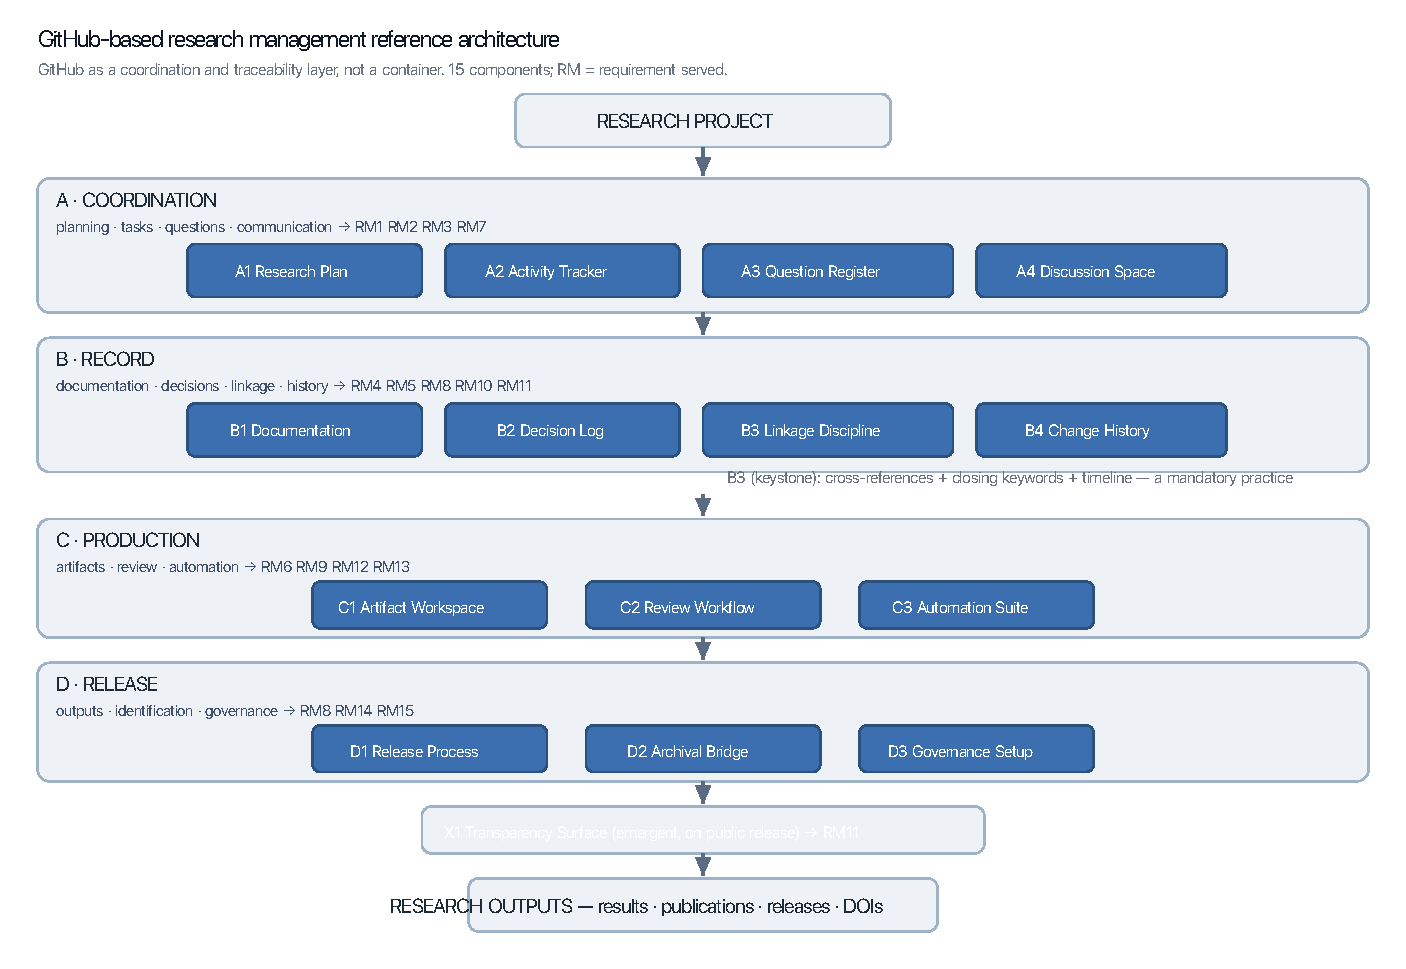
\includegraphics[width=\textwidth]{figures/fig3_architecture.pdf}
\caption{GitHub-based research management reference architecture (RQ4): five layers, fifteen components. GitHub acts as a coordination and traceability layer; large data, computational environments, persistent identifiers and institutional governance remain external and are linked by reference.}\label{fig:arch}
\end{figure}

\begin{figure}[h]
\centering
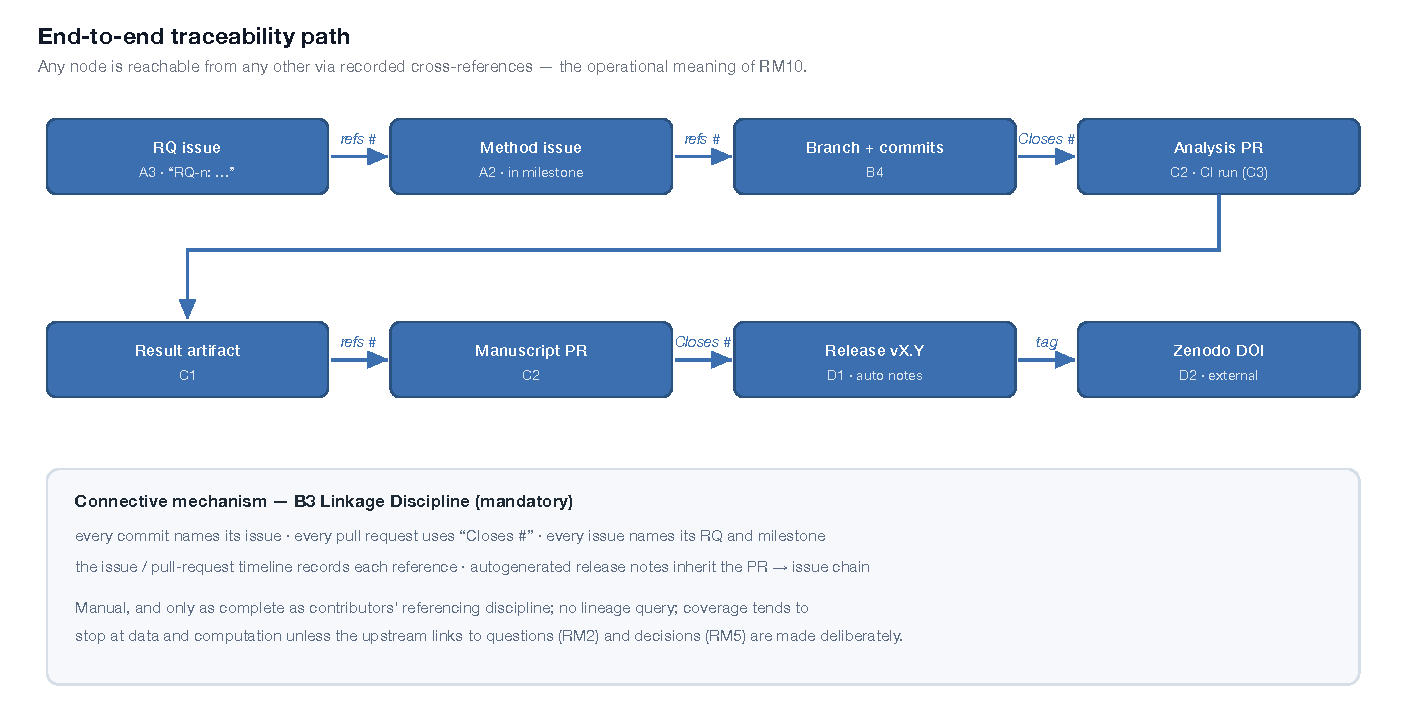
\includegraphics[width=\textwidth]{figures/fig4_traceability.pdf}
\caption{End-to-end traceability path produced by the linkage-discipline convention: a research-question issue is referenced by the method issue, whose branch and commits feed a reviewed pull request, whose result feeds the manuscript and a tagged release archived with a DOI. Any node is reachable from any other via recorded cross-references.}\label{fig:trace}
\end{figure}

\begin{table}[h]
\caption{Framework evaluation on six dimensions (RQ5), 0--2 scale, from the self-referential case study, after the repository was made public and one full issue-to-release cycle was run. ``Observed'' marks sub-scores evidenced by the actual repository state.}\label{tab:eval}
\begin{tabular}{@{}llc@{}}
\toprule
Dimension & Basis & Score \\
\midrule
E1 Requirement coverage & design-support & 2.00 \\
E2 Traceability         & observed & 1.75 \\
E3 Documentation        & observed & 2.00 \\
E4 Organization         & observed & 2.00 \\
E5 Transparency         & observed & 2.00 \\
E6 Usability            & observed & 1.50 \\
\midrule
Overall (21 sub-scores) & & \textbf{1.86} \\
Overall, observed only (20) & & 1.85 \\
\botrule
\end{tabular}
\end{table}

\begin{table}[h]
\caption{Fragmented workflow versus the GitHub-based framework (RQ5).}\label{tab:comparison}
\begin{tabular}{@{}p{2.4cm}p{4.6cm}p{4.6cm}@{}}
\toprule
Dimension & Fragmented workflow & GitHub-based framework \\
\midrule
Task traceability & tasks disconnected from the artifacts they produce & issues plus board plus closing keywords bind task to commit to pull request \\
Decision traceability & decisions in email and notes, rationale lost & numbered decision log plus decision issue, with rationale and affected artifacts \\
Version traceability & files renamed ``final''; no history & Git line-level history, diff, restore, tags \\
Documentation & scattered documents; drift; no history & version-controlled Markdown from project start, with per-folder READMEs \\
Research provenance & no systematic link between question, data and result & cross-references and timelines assemble the chain; release notes inherit it \\
Project visibility & known only to the email loop & public repository plus status, activity log and changelog \\
\botrule
\end{tabular}
\end{table}


\section{Discussion}\label{sec:discussion}

\subsection{Principal findings}\label{sec:d-principal}

The study's central result is a convergence. The gap identified bibliometrically in RQ1 --- the literature under-serves idea and question formulation, planning and decision traceability --- and the gap measured in RQ3 --- GitHub supports those same requirements at 1.67 against 2.50 for the rest --- are the same gap, reached by two independent routes. GitHub covers the execution-to-output span of the research lifecycle well and the upstream, research-specific layer poorly; the partiality is systematic, not incidental.

\subsection{GitHub as a coordination and traceability layer}\label{sec:d-layer}

Where research work can be expressed as files under version control, discrete tasks, branch-and-review changes and event-triggered automation, GitHub offers mature, purpose-built support, and the self-referential implementation confirms that this layer is low-cost: a full plan of record, twenty-six logged decisions and a reproducible analysis pipeline were produced with negligible overhead on the record layer, and the one full issue-to-release cycle run over the study's own backlog added only modest per-item effort for a solo author. Where the object of management is the evolving intellectual process --- the questions asked, the choices made and why --- GitHub offers only generic features on which a discipline must be imposed. The framework's contribution is to name that discipline: a mandatory linkage convention and three record conventions that make a plain repository into a traceable one. Even so, the differentiator requirements remain Partial or Limited; the framework maps the gap rather than closing it.

\subsection{Which lifecycle stages benefit}\label{sec:d-lifecycle}

Both the literature and GitHub's coverage are weakest at the earliest stages. The execution-to-output span --- methods, data, analysis, results, manuscript, release --- benefits most, because its artifacts are files and its activities are changes. The idea, question and planning stages benefit least, because they are deliberative and their ``artifacts'' are decisions. This is where tool development and reporting standards --- for decision records and research-question provenance --- would have the most leverage.

\subsection{Practical implications}\label{sec:d-practical}

For an individual researcher or a small group, the practical recommendation is to adopt the record and version-control layer first: a version-controlled \texttt{docs} directory, a decision log and disciplined commit messages deliver most of the traceability benefit at little cost. The Issue, Project and Pull Request layer should be added when the project has collaborators, where its coordination value accrues and its overhead is justified. The 33-file template lowers the setup cost of both.

\subsection{Relationship with output-preservation workflows}\label{sec:d-relationship}

This study addresses the management of the research process; a complementary line of work addresses the preservation and persistent identification of research \emph{outputs} through GitHub, Zenodo and ORCID. The two are the upstream and downstream halves of one lifecycle: the framework's release and archival-bridge components hand a versioned, cross-referenced record to an external archive that assigns a DOI. GitHub-based process management extends, rather than replaces, the open-science tooling around outputs.

\subsection{Limitations}\label{sec:limitations}

Six limitations bound the findings. First, the framework maps the upstream gap but does not close it: RM1, RM2 and RM5 stay Partial or Limited even with the prescribed conventions. Second, the coordination layer's \emph{collaborative} benefit is unproven: it was run through once end to end, but under single-author conditions, so the multi-author value of RM6, RM7 and the Issue/Project/Pull Request layer --- review, communication, parallel work --- was not observed. Third, the evaluation is single-case and self-referential, and every coding step had a single human coder; an independent re-code of all 53 coded decisions agreed at 96\% ($\kappa$ 0.83--1.00) and left the reported figures unchanged, but a second independent human rater was not available, and the retrospective second-project instantiation shares this study's lead author. Fourth, the primary bibliometric corpus is OpenAlex plus arXiv; a Scopus and Web of Science cross-check (18{,}250 raw records) shares 22\% of its DOIs with the corpus, the divergence being a characterised precision tail of tool-citing papers rather than missed core literature, and the broadest-query precision is $\approx 0.94$. Fifth, roughly a third of the coverage rests on mandatory convention rather than native features, as the stricter-rubric mean of 2.13 shows. Sixth, GitHub is not a complete research infrastructure: persistent identifiers and preservation, computational environments, large datasets and institutional governance are all external.

\subsection{Future research}\label{sec:d-future}

Three directions follow. The retrospective, single-author template instantiation reported here establishes structural transfer to another discipline; a \emph{prospective}, multi-author instantiation on a project run from the start would test the coordination layer's collaborative value and usability under realistic conditions. Instrumenting the linkage-discipline convention --- automatically checking that commits, pull requests and issues cross-reference their research question and decisions --- would move provenance from a manual practice toward a verifiable one. And a bibliometric follow-up on the upstream stages specifically would quantify whether the idea/question/planning gap is beginning to close as AI-assisted planning and digital ethics platforms mature.


\section{Conclusions}\label{sec:conclusions}

GitHub can serve as an integrated coordination and traceability \emph{layer} for a substantial part of the scientific research lifecycle. It supports thirteen of fifteen literature-derived research management requirements at partial or better and seven directly, with none unsupported; it is strong from execution to output and for research that resembles software engineering; and it is weak for the upstream, research-specific traceability of questions, decisions and provenance --- the very requirements the literature also under-serves. Five requirements need complementary external infrastructure. A fifteen-component reference architecture, four mandatory conventions and a thirty-three-file template operationalise what GitHub covers, and a self-referential implementation shows that its documentation and version-control layer works at near-zero overhead while the collaborative value of its coordination layer remains to be demonstrated. GitHub maps the research-process-management gap rather than closing it, and it is best understood not as a replacement for research infrastructure but as the coordination and traceability layer that a fragmented set of research tools currently lacks.


\section*{Declarations}

\subsection*{Data and code availability}\label{sec:data-availability}
The study repository --- bibliographic corpus, coding sheets, requirement and mapping tables, reference architecture, reusable template and all analysis scripts --- is openly available at \url{https://github.com/telmomm/github-research-infrastructure-study} and archived on Zenodo, DOI \href{https://doi.org/10.5281/zenodo.22167500}{10.5281/zenodo.22167500} (software record, a new version deposited per release). A companion dataset record, DOI \href{https://doi.org/10.5281/zenodo.22173525}{10.5281/zenodo.22173525}, holds the Track~A bibliometric corpus, the processed datasets and the raw database retrieval exports. Every table and figure in this paper is regenerated from these inputs by a versioned script.

\subsection*{Competing interests}
The author declares no competing interests.

\subsection*{Funding}
This research received no specific grant from any funding agency in the public, commercial or not-for-profit sectors.

\subsection*{Ethics approval}
Not applicable. The study involves no human participants, human data or animals; the bibliographic corpus consists of publication metadata from public indexes.

\subsection*{Author contributions}
T.M.-M.\ conceived and designed the study, performed the analysis, developed the framework and template, and wrote the manuscript.


\bibliography{references}

\end{document}
